\interlude*<left,leftskip=7cm,>[rosenpass-dragon]<Tribulations \textasciitilde\ Tooling>{Oh These\\Proof Tools}<Vive la Révolution! Against the Bourgeoisie of Proof Assistants!>
\section{Section: Better proof tools}

\begin{frame}[T]{Pen and Paper}
  \begin{columns}[fullwidth,t]
    \begin{column}{.29\linewidth}
      \raisebox{\dimeval{-\height}}{
\includegraphics[width=\linewidth]{this-is-fine-crop.png}}\par\nointerlineskip
      
\includegraphics[width=\linewidth]{this-is-not-fine-crop.jpg}%
    \end{column}
    \hfill
    \begin{column}{.68\linewidth}
      \small

\begin{description}[]
\item[{Bellare and Rogaway: [BR06]}]\leavevmode\newline many \enquote{essentially unverifiable} proofs, \enquote{crisis of rigor}

\item[{Halevi: [Hal05]}]\leavevmode\newline
	some reasons are social,
but \enquote{our proofs are truly complex}

%\item[{Joseph Jaeger: [ProTeCS 2024, Workshop at Eurocrypt]}]\leavevmode\newline
%technical and social reasons
%why and for whom do we write proofs?

%\item[We'd like to add:]\leavevmode\newline
%pen-and-paper proofs are hard to maintain, update, reuse
%especially for 3rd parties

%Can proofs become part of a continuous engineering effort?
\end{description}
    \end{column}
  \end{columns}
\end{frame}

\setbeamercolor{overlaybox}{bg=white}
\begin{frame}{Symbolic Modeling of Rosenpass}
  \begin{columns}[c]
    \begin{column}{.5\linewidth}
     \hspace*{-\UseName{beamer@leftmargin}}\rlap{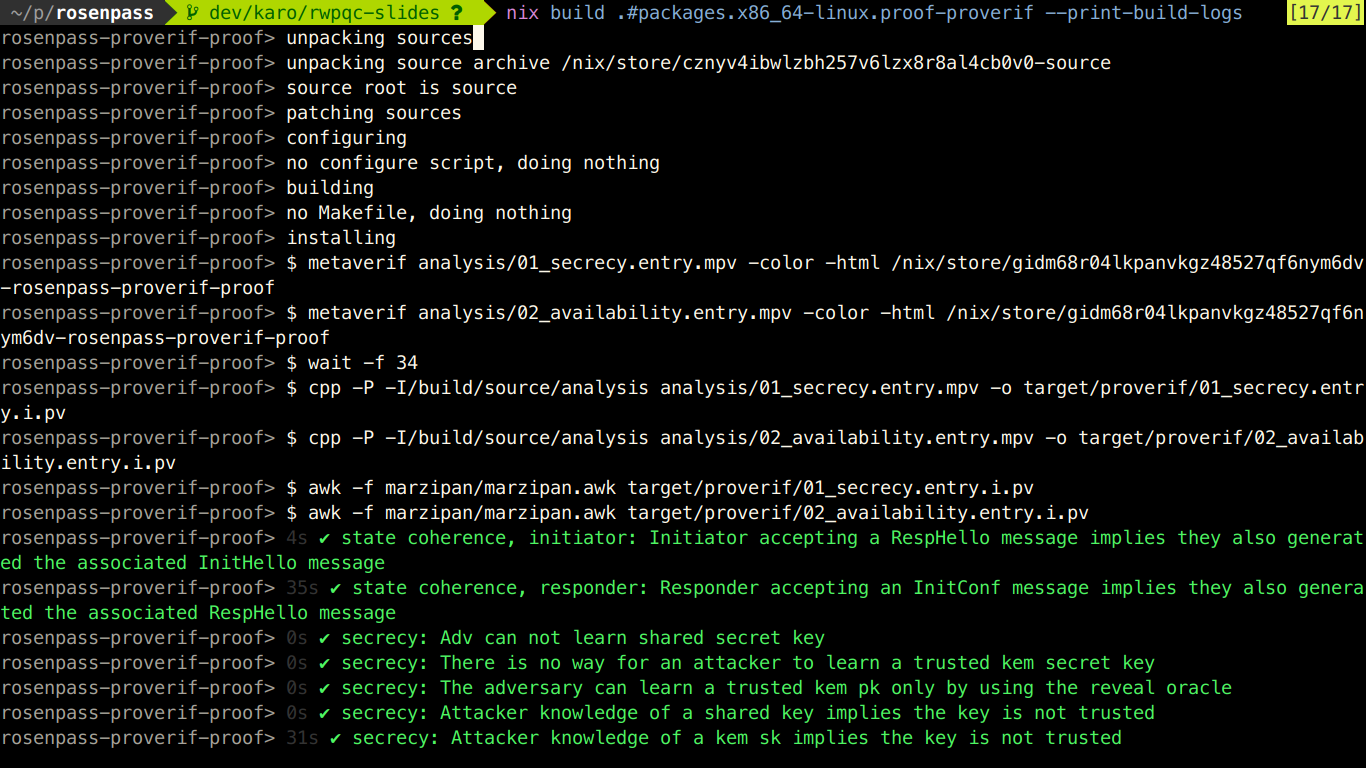
\includegraphics[keepaspectratio,height=\defaultframetextheight]{2023-03-20-symbolic-analysis-screenshot.png}}
    \end{column}%
	  %\pause
    \begin{column}{.5\linewidth}
    \begin{beamercolorbox}[colsep*=1ex,ht=\dimeval{\defaultframetextheight+2pt}]{overlaybox}
      \begin{itemize}
        \item symbolic modeling using ProVerif
        \item proofs treated as part of the codebase
        \item uses a model internally that is based on a fairly comprehensive Maximum Exposure Attacks (MEX) variant
        \item covers non-interruptability (resistance to disruption attacks)
        \item mechanized proof in the computational model is an open issue
      \end{itemize}
  \end{beamercolorbox}
    \end{column}
  \end{columns}
\end{frame}




% \begin{frame}{Friction \& Frustration for the Working Cryptographer}
%   \textbf{Tooling}
%   \begin{itemize}
%     \item Syntax highlighting, favorite editor
%     \item Engineering for large models: syntax rewriting, syntactic sugar, macros
%     \item Comfortable tooling to inspect intermediate games (CryptoVerif)
%   \end{itemize}
%   \vspace{1em}
%   \textbf{Documentation:} Often incomplete; step from example to research too big\\[.8em]

%   \textbf{Output:} hard to understand for non-experts\\[.8em]

%   \textbf{Input Language:} Unintuitive? Inaccessible? Mixed signals!\\[.8em]

%   \textbf{Proof Language:} not enough flexibility and leeway compared to pen-and-paper
%   \begin{itemize}
%     \item hand-waving, unsafe blocks
%       % pen-and-paper get way more leeway, mechanized proofs are often all or nothing
%     \item support for incremental process
%   \end{itemize}
% \end{frame}



% \begin{frame}{The Day Language Came into My Life}

%   %$\dots$ and mechanised proofs have not covered this thus far.

%   %\vspace{5em}

%   \blockquote[Helen Keller (1880--1968) in The Day Language Came into My Life]{
%     Everything had a name, and each name gave birth to a new thought.
%   }

% % We do not want to be typecast into people who just do usability or accessibility

% % language creates awareness, consciousness

% % neces. prerequisite

% % in order to be able to reason mathematically

% % math is the process of giving, of express math
% % concepts in the form of language
% %

% % math is something fundamentally kommunikatives

% % that's an aspect that mechanised proofs haven't covered thus far

% % Everything had a name, and each name gave birth to a new thought.
% % --- Helen Keller (1880--1968) in The Day Language Came into My Life


% % https://www.pval.org/cms/lib/NY19000481/Centricity/Domain/105/The%20Day%20Language%20Came%20into%20my%20Life.pdf

% \end{frame}










\begin{frame}{Rosenpass going Rube-Goldberg}
  \begin{columns}[fullwidth]
    \begin{column}{.7\linewidth}
      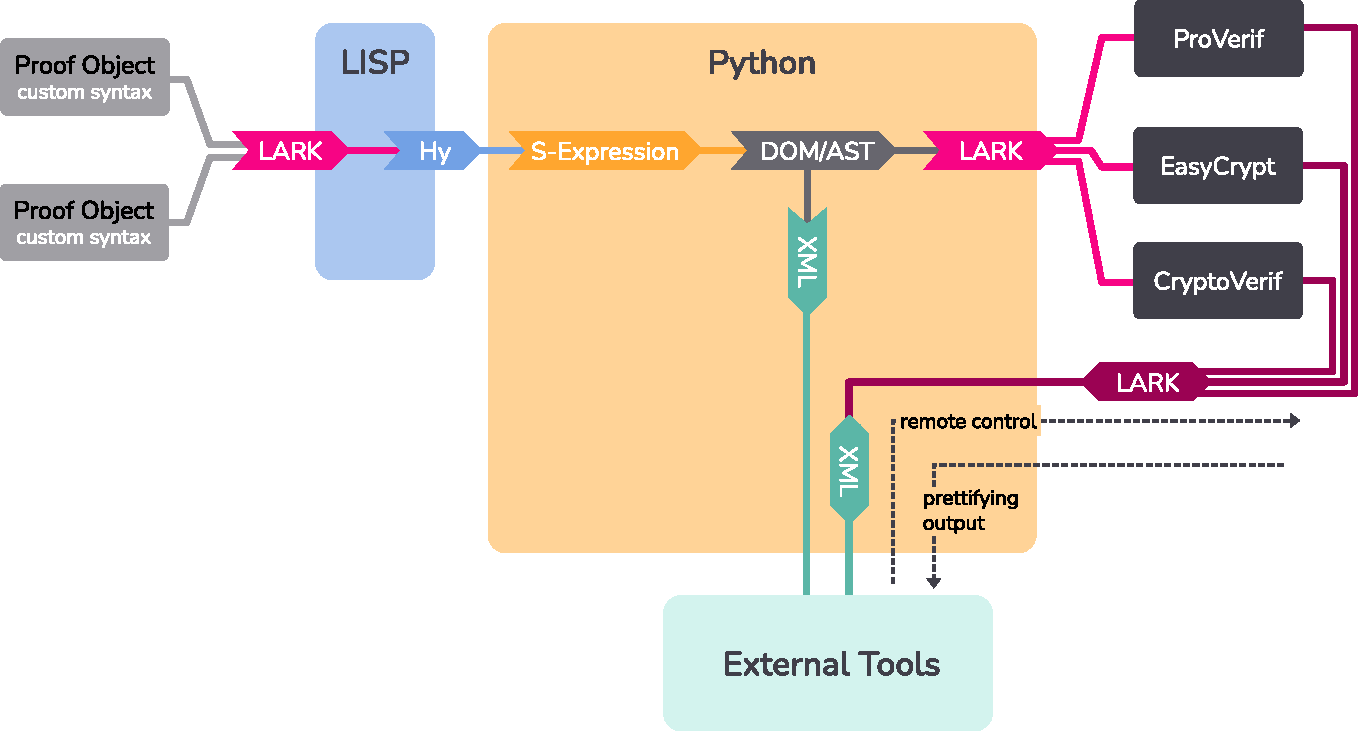
\includegraphics[width=\linewidth]{python-proofs.pdf}
    \end{column}\hfill
    \begin{column}{.28\linewidth}
\stretchcolumn{
      \textbf{We will} build a framework around existing tools
      \vfil

      \textbf{Keep} expressivity and preciseness

      \vfil
      \textbf{Generate \& Parse} their languages

      \vfil
      \textbf{Make these tools available} to other ecosystems using Python, Lisp, XML

	\vfil
}
    \end{column}

  \end{columns}
\end{frame}
